\chapter{Cadre général du projet et étude de l'existant}

Ce premier chapitre pose le cadre dans lequel s'inscrit ce projet de fin d'études. Il présente l'organisme d'accueil et le contexte bancaire dans lequel la plateforme développée doit s'intégrer, avant d'exposer la problématique et les objectifs qui en découlent. Un état des lieux des pratiques existantes et de leurs limites conduit ensuite à la solution proposée et à la méthodologie retenue pour la mener à bien, méthodologie dont les chapitres suivants détaillent la mise en œuvre effective.

\section{Présentation de l'organisme d'accueil}

\subsection{Présentation du groupe EY}

EY est un des leaders mondiaux de l'audit, du conseil, de la fiscalité et du droit, ainsi que des transactions. Le groupe inscrit son activité dans un objectif de confiance : la qualité de ses services vise à soutenir la fiabilité de l'économie et des marchés financiers, pour les entreprises comme pour les institutions publiques qu'il accompagne. Il rassemble environ 400~000 professionnels répartis dans près de 750 bureaux à travers 152 pays. Ses activités sont organisées autour de quatre lignes de services : Assurance, Consulting, Tax et Strategy and Transactions.

\begin{figure}[htbp]
    \centering
    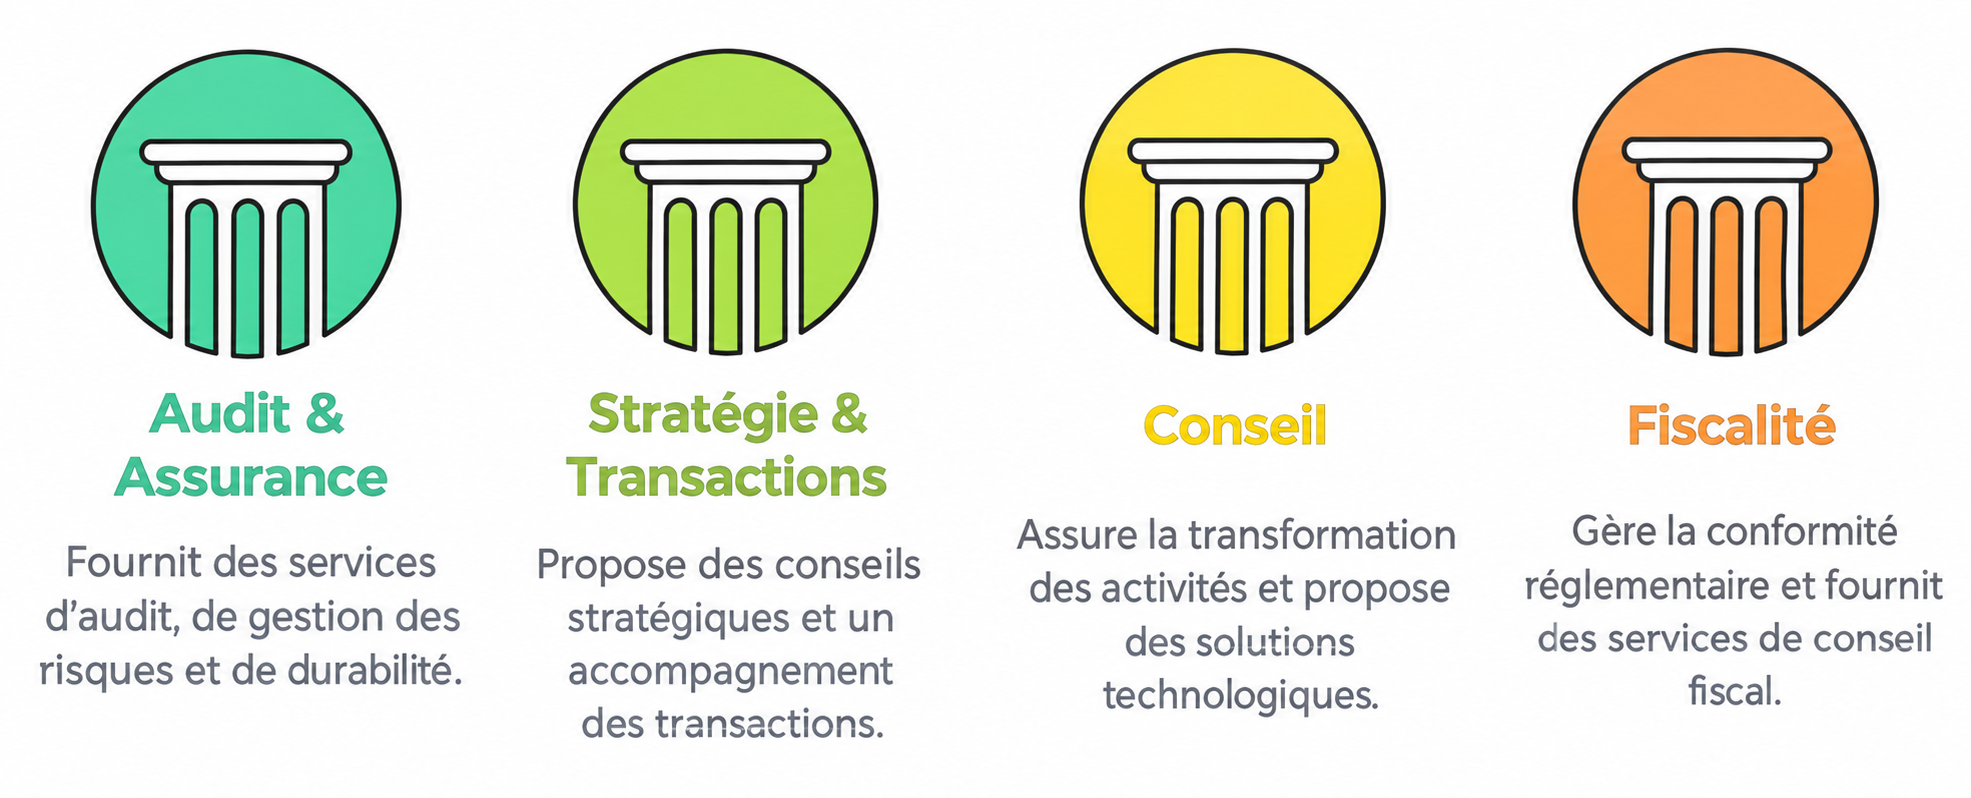
\includegraphics[width=0.25\textwidth]{figures/ey_logo.png}
    \caption{Logo du groupe EY \parencite{EYFY26}.}
    \label{fig:ey-logo}
\end{figure}

\subsection{Présentation d'EY Tunisie}

En Tunisie, EY est implanté depuis 1987 à travers son bureau de Tunis, sous la dénomination AMC Ernst \& Young. Le bureau compte plus de 900 professionnels, dont 23 associés, et couvre une dizaine de secteurs d'activité. Il y mène chaque année plus de 600 missions, couvrant une trentaine de pays. EY Tunisie y a notamment mis en place le premier laboratoire EY Cyber \& RPA en Tunisie, consacré à la cybersécurité et à l'automatisation robotisée des processus.

\subsection{Organisation et domaines d'activité}

L'activité d'EY Tunisie est organisée autour des quatre mêmes lignes de services qu'au niveau du groupe, présentées à la figure~\ref{fig:ey-lignes-service}. L'Assurance regroupe l'audit et les services associés, notamment en matière de risques financiers et de durabilité, au service de la fiabilité et de la transparence de l'information des clients. Le Consulting accompagne la transformation des organisations par la technologie, les données et l'intelligence artificielle, et couvre également des domaines tels que la cybersécurité et l'ingénierie digitale. La ligne Tax prend en charge la conformité fiscale des entreprises ainsi que le conseil en fiscalité internationale et en droit social. Strategy and Transactions, enfin, intervient dans les opérations de transaction, l'évaluation financière, les stratégies de croissance et les opérations de restructuration.

\begin{figure}[htbp]
    \centering
    
\includegraphics[width=0.85\textwidth]{figures/ey_quatre_lignes_service.png}
    \caption{Les quatre lignes de services d'EY Tunisie \parencite{EYFY26}.}
    \label{fig:ey-lignes-service}
\end{figure}

\subsection{Présentation de l'entité d'accueil}

Le stage à l'origine de ce rapport a été réalisé au sein de la ligne Consulting, et plus précisément de l'entité AI \& Data. C'est dans ce cadre qu'a été confiée la mission de gestion du risque de crédit bancaire présentée dans ce rapport.

\section{Contexte général du projet}

Le crédit constitue l'un des principaux leviers de financement de l'activité économique : il permet à des particuliers et à des entreprises de disposer de ressources qu'ils rembourseront progressivement, pour financer un investissement, une activité ou une consommation qu'ils ne pourraient pas couvrir avec leurs seules ressources immédiates. Pour la banque qui l'accorde, chaque crédit représente à la fois une source de revenus, à travers les intérêts perçus, et une exposition à un risque, celui de ne pas être intégralement remboursée. Développer les financements accordés tout en maîtrisant le risque associé constitue ainsi un équilibre que chaque banque doit rechercher en permanence, et qui conditionne directement sa solidité financière dans la durée.

Cet arbitrage repose sur quelques notions centrales. Le risque de crédit désigne la possibilité qu'un emprunteur ne respecte pas, en tout ou en partie, ses engagements de remboursement. Lorsque ce risque se matérialise, il se traduit par une perte, dont une partie est anticipée dès l'octroi du crédit : on parle alors de perte attendue, usuellement rapprochée de trois composantes : la probabilité de défaut de l'emprunteur (PD, \emph{Probability of Default}), la part de l'exposition qui ne serait pas recouvrée en cas de défaut (LGD, \emph{Loss Given Default}) et le montant de cette exposition au moment du défaut (EAD, \emph{Exposure at Default}), soit, sous une forme simplifiée, la perte de crédit attendue (ECL, \emph{Expected Credit Loss}) peut être exprimée par la relation $ECL \approx PD \times LGD \times EAD$. Cette expression donne une intuition de la relation entre ces trois composantes ; elle ne représente pas l'ensemble des modalités de calcul prévues par la norme IFRS 9, présentée ci-après. Au-delà de cette perte attendue, la banque doit également se prémunir contre des pertes inattendues, plus rares mais potentiellement plus importantes : c'est notamment le rôle des fonds propres, qui permettent à la banque d'absorber ces pertes et de préserver sa solvabilité. La rentabilité d'un crédit dépend ainsi non seulement des revenus qu'il génère, mais aussi du coût du risque qu'il représente et du capital qu'il immobilise.

Cette gestion du risque de crédit ne relève pas uniquement de choix internes à la banque : elle s'inscrit dans un cadre réglementaire qui en encadre la mesure et le provisionnement. La norme comptable \textsc{IFRS 9}, publiée par l'\textit{International Accounting Standards Board} et entrée en vigueur le 1er janvier 2018, repose sur un modèle général de dépréciation qui distingue trois catégories d'expositions, appelées \emph{stages} \parencite{IASB2014IFRS9}. Les expositions dont la qualité de crédit ne s'est pas dégradée de façon significative depuis leur comptabilisation initiale (stage 1) donnent lieu à la comptabilisation des pertes de crédit attendues associées aux défauts susceptibles de survenir au cours des douze mois suivant la date de clôture. Dès qu'une augmentation significative du risque de crédit est constatée depuis la comptabilisation initiale (SICR, \emph{Significant Increase in Credit Risk}, stage 2), ou \emph{a fortiori} lorsque l'exposition est dépréciée pour risque de crédit (stage 3), la provision doit couvrir la perte attendue sur toute la durée de vie restante de l'exposition, ce qui peut en accroître le montant, puisque l'horizon de calcul couvre désormais toute la durée de vie restante de l'exposition. À ce cadre comptable s'ajoute un cadre prudentiel, issu des accords de Bâle et porté par le \textit{Basel Committee on Banking Supervision}, qui définit des exigences minimales de fonds propres, notamment calculées à partir des actifs pondérés par les risques, afin de renforcer la capacité des banques à absorber les pertes \parencite{BCBS2017Basel3}. Ce capital réglementaire, calculé selon des règles communes à l'ensemble des établissements soumis à ces accords, ne se confond pas avec le capital économique qu'une banque peut par ailleurs estimer en interne pour ses propres besoins de pilotage.

Le projet présenté dans ce rapport s'inscrit dans cet environnement bancaire, financier et réglementaire. Il couvre deux niveaux d'analyse complémentaires : l'évaluation d'une nouvelle demande de crédit, désignée dans la suite du rapport par le terme \emph{Origination}, et le suivi d'un portefeuille de crédits déjà accordés, désigné par \emph{Portfolio Analytics}.

\section{Problématique et objectifs}

\subsection{Constat et formulation de la problématique}

La gestion du risque de crédit implique plusieurs dimensions complémentaires : l'évaluation du risque associé à un financement, l'estimation des pertes potentielles qui peuvent en résulter, la prise en compte du capital nécessaire pour absorber les pertes inattendues et l'appréciation de la rentabilité qu'il procure à la banque. Ces dimensions interviennent à différentes étapes du cycle de vie d'un crédit, depuis l'étude d'une nouvelle demande jusqu'au suivi, dans la durée, des financements déjà accordés.

La problématique à laquelle répond ce projet peut ainsi être formulée de la façon suivante : comment mettre en relation l'évaluation du risque de crédit et l'analyse de la rentabilité, afin d'éclairer à la fois la décision d'octroi d'un nouveau crédit et le suivi d'un portefeuille de crédits déjà accordés ?

\subsection{Objectif général}

L'objectif général de ce projet est de concevoir une plateforme d'aide à la décision permettant d'intégrer les dimensions du risque et de la rentabilité dans deux contextes complémentaires : l'évaluation des nouvelles demandes de crédit et le suivi des portefeuilles de crédits existants.

\subsection{Objectifs spécifiques}

Cet objectif général se décline en plusieurs objectifs spécifiques :

\begin{itemize}
    \item évaluer le risque associé à une nouvelle demande de crédit ;
    \item estimer les pertes attendues et prendre en compte le capital nécessaire à l'analyse de la rentabilité du dossier ;
    \item produire des éléments d'aide à la décision pour l'octroi des financements ;
    \item suivre et analyser, pour un portefeuille de crédits déjà accordés, le risque, les pertes attendues, le capital mobilisé et la rentabilité dans la durée ;
    \item présenter ces résultats sous forme d'indicateurs et d'analyses directement exploitables par les utilisateurs métier.
\end{itemize}

\section{Étude et critique de l'existant}

Pour situer le projet par rapport à l'existant, cette section compare trois solutions commerciales reconnues sur le marché de la gestion du risque de crédit : SAS, Moody's Analytics et FICO. Plutôt que de dresser un inventaire exhaustif de leurs fonctionnalités, l'analyse qui suit dégage, pour chacune, son positionnement, ses apports documentés et ses limites telles qu'elles ressortent de leur documentation officielle (tableau~\ref{tab:etude-existant}). Cette analyse comporte une limite méthodologique qu'il convient d'assumer explicitement : une fonctionnalité non mentionnée dans la documentation publique consultée ne peut être considérée comme inexistante dans l'offre réelle de l'éditeur.

\begin{table}[htbp]
    \centering
    \footnotesize
    \caption{Étude critique de trois solutions commerciales de gestion du risque de crédit.}
    \label{tab:etude-existant}
    \begin{tabular}{p{1.8cm}p{2.7cm}p{3cm}p{3.5cm}p{3.3cm}}
        \toprule
        \textbf{Solution} & \textbf{Positionnement} & \textbf{Points forts documentés} & \textbf{Limites et points de vigilance} & \textbf{Enseignements pour le projet} \\
        \midrule
        SAS \parencite{SASIFRS9} &
        Provisionnement et conformité IFRS 9 (ECL, classification par \emph{stage}). &
        Modèles PD/LGD préconstruits ; automatisation du calcul des ECL par scénario. &
        Documentation centrée sur le provisionnement comptable, sans détail sur le capital réglementaire ou la rentabilité par dossier. &
        Confirme la maturité attendue sur l'IFRS 9, à relier explicitement à la rentabilité du dossier. \\
        \addlinespace
        Moody's Analytics \parencite{MoodysIFRS9} &
        Souscription, surveillance de portefeuille et modélisation IFRS 9, via plusieurs produits dédiés. &
        Scénarios macroéconomiques sur plus de 70 pays ; \emph{staging} IFRS 9 documenté ; usage cité pour le capital interne au risque. &
        Les produits sont présentés séparément dans la documentation consultée, qui ne met pas explicitement en évidence un flux unique reliant octroi et suivi de portefeuille. &
        Couverture fonctionnelle large, que le projet cherche à relier dans un même processus. \\
        \addlinespace
        FICO \parencite{FICOOriginations} &
        Décisionnel d'octroi : stratégies combinant risque de crédit et détection de fraude. &
        Configuration des stratégies en \emph{low-code} ; risque et fraude dans une même couche décisionnelle. &
        Documentation centrée sur l'octroi, sans détail sur le suivi du portefeuille dans la durée. &
        Confirme l'intérêt d'un décisionnel d'octroi structuré, complété par un suivi de portefeuille. \\
        \bottomrule
    \end{tabular}
\end{table}

Cette comparaison met en évidence des positionnements complémentaires : SAS met l'accent sur le provisionnement IFRS 9, Moody's Analytics propose plusieurs solutions couvrant différentes dimensions de la gestion du risque, tandis que FICO se concentre notamment sur le décisionnel d'octroi. Les documentations étudiées ne mettent toutefois pas explicitement en évidence une démarche réunissant l'évaluation du risque, l'analyse de la rentabilité, la décision d'octroi et le suivi du portefeuille dans un même processus. Ce constat, limité aux informations publiquement documentées, permet de situer le positionnement du projet présenté dans ce rapport.

\section{Solution proposée}

La solution proposée dans ce rapport est une plateforme d'aide à la décision qui met en regard, pour un crédit comme pour un portefeuille déjà constitué, le risque qu'il représente et la rentabilité qu'il procure à la banque, occupant ainsi l'espace mis en évidence à l'issue de l'étude de l'existant. Elle se décline en deux volets complémentaires : \emph{Origination}, qui couvre l'évaluation d'une nouvelle demande de crédit jusqu'à la décision d'octroi, et \emph{Portfolio Analytics}, qui couvre le suivi d'un portefeuille de crédits déjà accordés. Les deux volets s'appuient sur un socle commun d'évaluation du risque, sans que leurs calculs soient nécessairement identiques : le capital mobilisé, par exemple, ne se détermine pas selon le même mécanisme pour un dossier individuel et pour un portefeuille.

Dans les deux cas, la plateforme suit le même enchaînement fonctionnel : évaluation du risque, estimation des pertes attendues, puis prise en compte du capital nécessaire pour absorber d'éventuelles pertes inattendues et de la rentabilité du financement, pour aboutir à un résultat exploitable. Ce résultat prend la forme d'une décision d'octroi assortie de ses justifications pour \emph{Origination}, et d'un ensemble d'indicateurs portant sur le risque, les pertes attendues, le capital mobilisé et la rentabilité du portefeuille, calculés à intervalles réguliers pour \emph{Portfolio Analytics}, indépendamment des décisions d'octroi : ce suivi ne découle pas automatiquement de chaque décision. Les besoins qui en découlent sont précisés au chapitre~2, les traitements métier et techniques aux chapitres~3 à 6, et l'architecture de la plateforme au chapitre~5.

\section{Méthodologie utilisée}

\subsection{Principes d'une démarche itérative et incrémentale}

Une démarche itérative et incrémentale repose sur deux principes distincts, souvent évoqués ensemble mais qui ne se confondent pas \parencite{LarmanBasili2003}. Le principe itératif consiste à revenir, au fil de cycles de travail successifs, sur des éléments déjà réalisés, afin de les affiner ou de les corriger à la lumière de nouveaux résultats. Le principe incrémental consiste, de son côté, à construire la solution par ajouts progressifs : chaque étape complète ce qui a déjà été réalisé, sans nécessairement tout reprendre depuis le début. Associés, ces deux principes permettent de faire évoluer une solution progressivement, tout en conservant la possibilité de revenir sur des choix antérieurs lorsque leur vérification le justifie, comme l'illustre la figure~\ref{fig:cycle-iteratif}. C'est selon ces deux principes que ce projet a été conduit.

\begin{figure}[htbp]
    \centering
    \begin{tikzpicture}[
        box/.style={draw, rounded corners, align=center, minimum width=3.4cm, minimum height=1.2cm, font=\footnotesize, fill=gray!10},
        arrow/.style={-{Latex[length=2.5mm]}, thick}
    ]
        \node[box] (top) at (0,3) {Réalisation incrémentale\\(ajout d'un élément)};
        \node[box] (right) at (4,0) {Vérification};
        \node[box] (bottom) at (0,-3) {Ajustement itératif\\(reprise si nécessaire)};
        \node[box] (left) at (-4,0) {Consolidation};
        \node[align=center, font=\footnotesize\itshape] at (0,0) {Évolution progressive\\de la solution};
        \draw[arrow] (top.east) to[bend left=25] (right.north);
        \draw[arrow] (right.south) to[bend left=25] (bottom.east);
        \draw[arrow] (bottom.west) to[bend left=25] (left.south);
        \draw[arrow] (left.north) to[bend left=25] (top.west);
    \end{tikzpicture}
    \caption{Schéma illustrant le principe itératif et incrémental retenu pour ce projet (illustration personnelle).}
    \label{fig:cycle-iteratif}
\end{figure}

\subsection{Phases de la démarche suivie}

Le travail s'est organisé autour de quatre grandes phases, résumées dans le tableau~\ref{tab:phases-demarche}. Ces phases ne se sont pas succédé de façon strictement linéaire : une vérification menée dans l'une d'elles pouvait remettre en cause une décision prise lors d'une phase antérieure, qu'il fallait alors reprendre avant de poursuivre.

\begin{table}[htbp]
    \centering
    \footnotesize
    \caption{Phases de la démarche suivie.}
    \label{tab:phases-demarche}
    \begin{tabular}{p{3.2cm}p{5cm}p{6cm}}
        \toprule
        \textbf{Phase} & \textbf{Objectif} & \textbf{Travaux réalisés} \\
        \midrule
        Compréhension du besoin et cadrage &
        Analyser le contexte métier du risque de crédit et délimiter le périmètre du projet. &
        Étude du cadre réglementaire et financier, identification des besoins, définition des deux volets du projet. \\
        \addlinespace
        Préparation et constitution des données &
        Réunir et préparer les données nécessaires à l'évaluation du risque. &
        Nettoyage des données réelles disponibles, génération de données synthétiques de comportement de défaut, calibration et vérification de ces données. \\
        \addlinespace
        Conception et développement des traitements &
        Concevoir et développer les traitements d'évaluation du risque, de quantification financière et d'aide à la décision. &
        Construction des modèles de score de crédit, calculs de pertes attendues, de capital et de rentabilité, mécanismes de décision et de pilotage. \\
        \addlinespace
        Vérification et amélioration &
        Évaluer la cohérence et la fiabilité des traitements développés. &
        Audits de cohérence, tests sur les traitements métier et sur leur intégration. \\
        \bottomrule
    \end{tabular}
\end{table}

Deux vérifications menées au cours de ces phases illustrent concrètement cette démarche. Lors de la préparation des données, un audit du processus de génération des données synthétiques du segment Entreprises a mis en évidence un taux cible de défaut trop élevé au regard du comportement attendu du segment ; ce taux a été revu à la baisse et la génération des données reprise en conséquence. Lors de la conception des traitements, l'évaluation d'un des algorithmes candidats au score de crédit du segment Particuliers, sur un jeu de test organisé selon un découpage temporel, a révélé une forte dégradation de ses performances, mettant en évidence une capacité de généralisation insuffisante sur des données temporellement plus récentes ; cet algorithme a été écarté du choix final au profit des deux autres candidats retenus. Une correction motivée par l'une des vérifications de la dernière phase a par ailleurs pu être répercutée sur des livrables antérieurs déjà considérés comme aboutis, lorsqu'elle concernait un élément qu'ils réutilisaient.

\subsection{Bénéfices de la démarche suivie}

Une démarche itérative et incrémentale est généralement présentée, dans les principes qui la définissent, comme permettant de détecter plus tôt les incohérences et les erreurs, de valider progressivement les choix retenus plutôt que de les découvrir en bloc en fin de projet, et de s'adapter à des exigences qui ne sont pas toutes connues ni figées dès le départ. Dans le cadre de ce projet, cette démarche a permis de confronter progressivement les choix effectués aux résultats obtenus et de les ajuster lorsque les vérifications le nécessitaient. Les reprises réalisées ont ainsi contribué à corriger les incohérences détectées et à renforcer la cohérence entre les différentes composantes de la plateforme. Elles ont également permis de fonder les décisions de développement sur des résultats contrôlés plutôt que sur des hypothèses non vérifiées.

\section*{Conclusion du chapitre}

Ce chapitre a situé le projet présenté dans ce rapport : réalisé au sein de l'entité AI \& Data d'EY Tunisie, il répond à un besoin de rapprocher l'évaluation du risque de crédit et l'analyse de la rentabilité, dans un environnement bancaire structuré par les normes IFRS 9 et Bâle. L'étude de trois solutions commerciales existantes a montré que les documentations consultées ne mettent pas explicitement en évidence une approche réunissant ces deux dimensions, aussi bien pour l'octroi d'un nouveau crédit que pour le suivi d'un portefeuille existant. C'est cet espace que la plateforme proposée, déclinée en deux volets complémentaires, \emph{Origination} et \emph{Portfolio Analytics}, cherche à occuper. Sa réalisation a suivi une démarche itérative et incrémentale, dont les phases et les ajustements ont été détaillés dans ce chapitre. Le chapitre suivant précise les besoins fonctionnels et non fonctionnels qui découlent de ce cadrage, ainsi que les utilisateurs auxquels la plateforme s'adresse.
